\chapter{Uno strumento orientato alla creaziene di configurazioni avanzate: l'evoluzione di \visualnetkit{}}\label{capitolo:evoluzione_visualnetkit}
\markboth{Uno strumento orientato alla creaziene di configurazioni avanzate}{}

Come abbiamo introdotto nel capitolo \ref{capitolo:arte} \visualnetkit{} offre un ottima flessibilità a livello architetturale grazie alla sua struttura modulare che si appoggia su \plugin{}, ma allo stesso tempo questa malleabilità è limitata dal potere espressivo dei singoli \plugin{}. Infatti, questi possono offrire il loro contributo introducendo solamente parametri aggiuntivi espressi sotto forma di una lista di coppie chiave-valore rappresentanti le informazioni che il \plugin{} andrà ad inserire all'interno dei template\footnote{Ogni ``template'' rappresenta il contenuto testuale che andrà scritto sul file di configurazione indicato dal \plugin{} stesso; se più \plugin{} vogliono scrivere sul medesimo file di configurazione, il sistema non fa altro che accodare i vari templates.} che produrrà.

In questo capitolo discuteremo di come \visualnetkit{} sia stato profondamente modificato per dare la possibilità ai vari \plugin{} di poter ``abbracciare'' praticamente la totalità delle tipologie dei file di configurazione dei vari servizi (Dns, HTTP, E-Mail, Zebra, SSH, ecc\ldots). Si discuterà d'apprima il problema analizzando alcune configurazioni avanzate di BGP e OSPF, e da questo si cercerà di estrapolare una struttura da poter descrivere all'interno dei vari \plugin{}. Successivamente si formalizzeranno i nuovi requisiti discutendo l'impatto di tali modifiche sul sistema attuale, ed in fine ci addentreremo in uno studio di ``Analisi Architetturale'' del nuovo sistema di gestione delle properties dei \plugin{}.

\section{Il problema delle configurazioni complesse}
Quando si ha a che fare con servizi complessi come Zebra\footnote{GNU Zebra è un software opensource che gestisce i protocolli di routing basati su TCP/IP. Supporta il protocollo BGP-4 come descritto nell'RFC-1771, come anche RIPv1, RIPv2 e OSPFv2.}, quasi sempre si ha a che fare anche con file di configurazione dall'alto potere espressivo e quindi potenzialmente complessi.

Andremo ora ad analizzare da vicino due esempi di configurazioni complesse in Zebra, in particolare nei protocolli BGP\footnote{Il \emph{Border Gateway Protocol} (BGP) è un protocollo di rete usato per connettere tra loro più router che appartengono a sistemi autonomi distinti e che vengono chiamati gateway.} e OSPF\footnote{Il protocollo \emph{Open Shortest Path First} (OSPF) è uno dei protocolli di instradamento più diffusi, che gestisce le tabelle di instradamento di una rete IP con il metodo del Link State.}, e cercheremo di trovare una possibile struttura comune che possa racchiuderli.

\subsection{Configurazione avanzata in BGP}
In questa sezione cerceremo di indivinuare una struttura comune in uno scenario reale, prendendo come esempio la configurazione BGP proposta in figura \ref{figura:bgp_conf_schema}.

\begin{figure}[!htb]
	\centering
	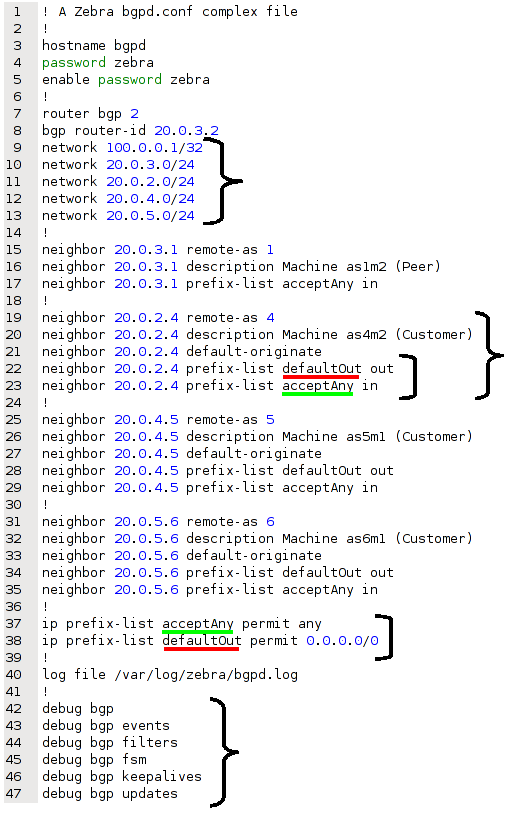
\includegraphics[width=10cm]{images/bgp_conf_schema.png}
	\caption{Una configurazione complessa di BGP.}
	\label{figura:bgp_conf_schema}
\end{figure}

Osservando la struttura del file di configurazione proposto, notiamo subito che vi è una struttura comune che può essere estrapolata e classificata. Senza considerare le righe $1\mapsto8$ che sono riconducibili ad una semplice lista di coppie chiave-valore, soffermiamoci alle righe $9\mapsto13$; qui troviamo le network annunciate dal router in questione e possiamo gia' identificare che tale struttura è una lista con cardinalità 0..n di coppie con chiave ``network'' e con valore uguale all'indirizzo IP più netmask che si vuole annunciare. Già in questo scenario una coppia chiave-valore (usata nella versione $1.0$ di \visualnetkit{}) non può essere utilizzata poiché solitamente le chiavi devono rimanere univoche.

Osserviamo ora le righe $15\mapsto35$ e soffermiamoci in particolare sulle righe $19\mapsto23$. Come descritto nella documentazione di Zebra\cite{ZEBRADOC} un ``peer'' ha la seguente sintassi:
\\
\\
\textbf{neighbor} \textit{peer} \textbf{remote-as} \textit{AS-Number}
\\
\textbf{neighbor} \textit{peer} \textbf{COMMAND}
\\
\\
dove \textbf{COMMAND} è uno dei comandi previsti da Zebra come ad esempio: \emph{description, default-originate, interface, version,} ecc\ldots nonché comandi atti al \emph{Peer Filtering} quali: \emph{discribuite-list, prefix-list, route-map,} ecc\ldots

\begin{figure}[!htb]
	\centering
	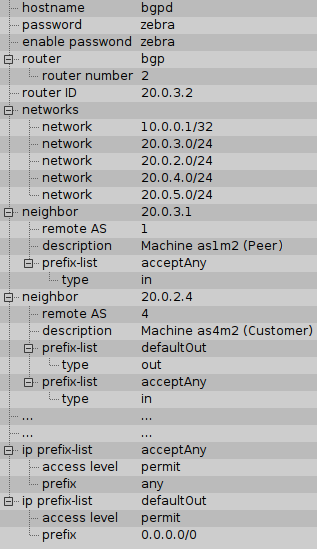
\includegraphics[width=6cm]{images/bgp_conf_tree.png}
	\caption{Configurazione complessa di BGP con struttura gerarchica.}
	\label{figura:bgp_conf_tree}
\end{figure}

Quindi, anche in questo caso è possibile raggruppare le varie definizioni dei ``vicini'' (neighbor) in una struttura gerarchica dove ogni neighbor ha una truttura composta da sotto proprietà, eventualmente con proprietà che si riferiscono a nodi esterni come nel nostro caso \emph{prefix-list} (righa $22-23$). Proprio partendo da queste due righe, possiamo identificare quindi proprietà correlate (simili al concetto di chiavi esterne in uno schema relazionale di basi di dati) a entità esterne; stiamo in definitiva affermando che quella che abbiamo davanti non è nient'altro che una struttura ad albero n-ario che possiede un enorme potere descrittivo, ma allo stesso tempo una struttura complessa da gestire e manipolare. In figura \ref{figura:bgp_conf_tree} viene mostrata la mappatura del file di configurazione in esame (figura \ref{figura:bgp_conf_schema}) in un albero n-ario.

Quella appena mostrata non è che una delle tante possibili interpretazioni di un file di configurazione in una struttura gerarchica. Solitamente ogni file di configurazione (soprattutto nei sistemi \emph{Unix like}) possiede una struttura che è riconducibile ad una con caratteristiche gerarchiche. Proprio verso questa direzione l'evoluzione che \visualnetkit{} ha avuto si è mossa, in particolare tranformando il vecchio modello chiave-valore delle proprietà dei \plugin{}, in uno altamente dinamico (con la possibilità di inserire e/o eliminare proprietà) con struttura annidata.

\subsection{Configurazione avanzata in OSPF}
Ora tenteremo di applicare quanto detto pocanzi ad un altro scenario reale che coinvolge il protocollo OSPF ed il suo file di configurazione. Prendiamo dunque in esame il file di configurazione mostrato in figura \ref{figura:ospf_conf}.

\begin{figure}[!htb]
	\centering
	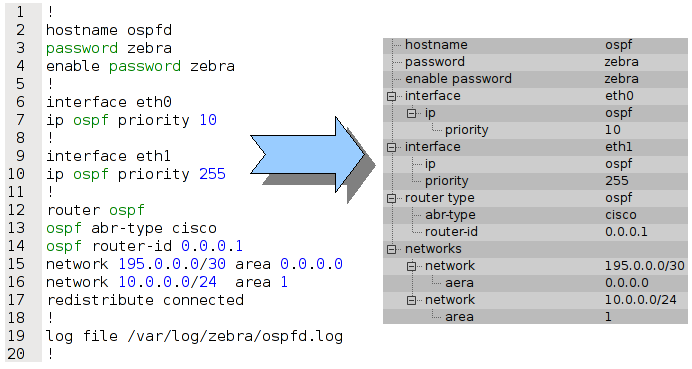
\includegraphics[width=12cm]{images/ospf_conf_schema_tree.png}
	\caption{Configurazione di OSPF e relativa vista gerarchica.}
	\label{figura:ospf_conf}
\end{figure}

Anche in questo caso possiamo procedere nel cercar di trasformare il contenuto del file di configurazione proposto, in una stuttura descritta da un albero n-ario. Iniziamo quindi ad analizzare il testo soffermandoci nelle righe $6\mapsto10$; possimo subito notare come quasta porzione abbia una struttura abbastanza uniforme - come descritto nella documentazione\cite{ZEBRADOC} - che può essere mappata all'interno di una struttura più auto descrittiva e gerarchica (figura \ref{figura:ospf_conf}).

Soffermiamoci ora sulle righe $15-16$ tralasciando le altre. In questo caso possiamo recavare una struttura ben precisa che nella documentazione di Zebra viene presentata nel seguente modo:
\\
\\
\textbf{network} \textit{a.b.c.d/m} \textbf{area} \textit{a.b.c.d}
\\
\textbf{network} \textit{a.b.c.d/m} \textbf{area} <\textit{0-4294967295}>
\\
\\
Naturalmente questi scenari sono soltanto alcuni dei tanti possibili contenuti che si possono trovare all'interno delle varie configurazioni, tuttavia abbiamo appena mostrato che qualunque siano le regole presenti nelle varie impostazioni dei servizi utilizzati, si riesce sempre a ricondurre questi ad una rappresentazione gerarchica talvolta anche complessa.

\section{Formalizzazione dei nuovi requisiti}

\section{Analisi architetturale}

\subsection{Definizione della nuova architettura per i \plugin{}}

\subsection{Il processo di sviluppo adottato}

